% Options for packages loaded elsewhere
\PassOptionsToPackage{unicode}{hyperref}
\PassOptionsToPackage{hyphens}{url}
%
\documentclass[
]{article}
\usepackage{lmodern}
\usepackage{amssymb,amsmath}
\usepackage{ifxetex,ifluatex}
\ifnum 0\ifxetex 1\fi\ifluatex 1\fi=0 % if pdftex
  \usepackage[T1]{fontenc}
  \usepackage[utf8]{inputenc}
  \usepackage{textcomp} % provide euro and other symbols
\else % if luatex or xetex
  \usepackage{unicode-math}
  \defaultfontfeatures{Scale=MatchLowercase}
  \defaultfontfeatures[\rmfamily]{Ligatures=TeX,Scale=1}
\fi
% Use upquote if available, for straight quotes in verbatim environments
\IfFileExists{upquote.sty}{\usepackage{upquote}}{}
\IfFileExists{microtype.sty}{% use microtype if available
  \usepackage[]{microtype}
  \UseMicrotypeSet[protrusion]{basicmath} % disable protrusion for tt fonts
}{}
\makeatletter
\@ifundefined{KOMAClassName}{% if non-KOMA class
  \IfFileExists{parskip.sty}{%
    \usepackage{parskip}
  }{% else
    \setlength{\parindent}{0pt}
    \setlength{\parskip}{6pt plus 2pt minus 1pt}}
}{% if KOMA class
  \KOMAoptions{parskip=half}}
\makeatother
\usepackage{xcolor}
\IfFileExists{xurl.sty}{\usepackage{xurl}}{} % add URL line breaks if available
\IfFileExists{bookmark.sty}{\usepackage{bookmark}}{\usepackage{hyperref}}
\hypersetup{
  hidelinks,
  pdfcreator={LaTeX via pandoc}}
\urlstyle{same} % disable monospaced font for URLs
\usepackage[margin=1in]{geometry}
\usepackage{graphicx,grffile}
\makeatletter
\def\maxwidth{\ifdim\Gin@nat@width>\linewidth\linewidth\else\Gin@nat@width\fi}
\def\maxheight{\ifdim\Gin@nat@height>\textheight\textheight\else\Gin@nat@height\fi}
\makeatother
% Scale images if necessary, so that they will not overflow the page
% margins by default, and it is still possible to overwrite the defaults
% using explicit options in \includegraphics[width, height, ...]{}
\setkeys{Gin}{width=\maxwidth,height=\maxheight,keepaspectratio}
% Set default figure placement to htbp
\makeatletter
\def\fps@figure{htbp}
\makeatother
\setlength{\emergencystretch}{3em} % prevent overfull lines
\providecommand{\tightlist}{%
  \setlength{\itemsep}{0pt}\setlength{\parskip}{0pt}}
\setcounter{secnumdepth}{-\maxdimen} % remove section numbering
\usepackage{float} \usepackage{caption} \captionsetup[table]{font=footnotesize} \captionsetup[figure]{font=footnotesize} \captionsetup[figure]{labelformat=empty} \captionsetup[table]{labelformat=empty} \usepackage{pdflscape} \newcommand{\blandscape}{\begin{landscape}} \newcommand{\elandscape}{\end{landscape}}
\usepackage{setspace}\onehalfspacing \usepackage{lineno}\linenumbers
\usepackage{booktabs}
\usepackage{longtable}
\usepackage{array}
\usepackage{multirow}
\usepackage{wrapfig}
\usepackage{float}
\usepackage{colortbl}
\usepackage{pdflscape}
\usepackage{tabu}
\usepackage{threeparttable}
\usepackage{threeparttablex}
\usepackage[normalem]{ulem}
\usepackage{makecell}

\author{}
\date{\vspace{-2.5em}}

\begin{document}

\raggedright

\textbf{Title:} Carbon cycling in mature and regrowth forests globally:
a macroecological synthesis based on the global Forest Carbon (ForC)
database

\textbf{Authors:}

Kristina J. Anderson-Teixeira\textsuperscript{1,2}*

Valentine Herrmann\textsuperscript{1}

Becky Banbury Morgan\textsuperscript{3}

Ben Bond-Lamberty\textsuperscript{4}

Susan C. Cook-Patton\textsuperscript{5}

Abigail E. Ferson\textsuperscript{1,6}

Jennifer C. McGarvey\textsuperscript{1}

Helene C. Muller-Landau\textsuperscript{1}

Maria M. H. Wang\textsuperscript{1,7}

\textbf{Author Affiliations:}

\begin{enumerate}
\def\labelenumi{\arabic{enumi}.}
\tightlist
\item
  Conservation Ecology Center; Smithsonian Conservation Biology
  Institute; National Zoological Park, Front Royal, VA 22630, USA
\item
  Center for Tropical Forest Science-Forest Global Earth Observatory;
  Smithsonian Tropical Research Institute; Panama, Republic of Panama
\item
  School of Geography, University of Leeds, Leeds, UK
\item
  Joint Global Change Research Institute, Pacific Northwest National
  Laboratory, College Park Maryland 20740, USA
\item
  The Nature Conservancy; Arlington VA 22203, USA
\item
  College of Natural Resources, University of Idaho; Moscow, Idaho
  83843, USA
\item
  Grantham Centre for Sustainable Futures and Department of Animal and
  Plant Sciences, University of Sheffield, Western Bank, Sheffield,
  South Yorkshire S10 2TN, UK
\end{enumerate}

*corresponding author:
\href{mailto:teixeirak@si.edu}{\nolinkurl{teixeirak@si.edu}}; +1 540 635
6546

\begin{verbatim}
## [1] 0
\end{verbatim}

\emph{NOTES TO COAUTHORS: }

\begin{itemize}
\tightlist
\item
  We're still finalizing the data (and adding some data). Outliers in
  plots will all be checked/ resolved, and we'll be able to pull in more
  data (GROA needs classification by dominant vegetation before it can
  be pulled in, and we're working on that)
\item
  ``\textbf{???}'' indicates a reference that we have entered in the
  .Rmd file, but not yet in the bibliography file. Don't worry about
  those. (However, places with ``REF'' need references)
\item
  bold/ italic text indicates places where I know we need to go back and
  revisit/ fill in info
\end{itemize}

\newpage

\hypertarget{summary}{%
\subsection{Summary}\label{summary}}

\emph{Background.} The fate of Earth's climate is closely linked to
forests, which strongly influence atmospheric carbon dioxide
(CO\textsubscript{2}) and climate through their influential role in the
global carbon (C) cycle. Synthetic understanding of global forest C
cycles is needed to constrain model estimates of forest feedbacks to
climate change and to more accurately quantify the influence of land use
decisions on climate.

\emph{Methods/Design.} Here, we draw from the Global Forest C Database,
ForC, to provide a macroscopic overview of C cycling in the world's
forests, giving special attention to stand age-related variation.
Specifically, we use 14847 ForC records from 874 geographic locations
representing 34 C cycle variables to characterize ensemble C budgets for
four broad forest types (tropical broadleaf evergreen, temperate
broadleaf, temperate conifer, and taiga), including estimates for both
mature and regrowth (age \textless100 years) forests. For regrowth
forests, we quantify age trends for all variables.

\emph{Review Results/ Synthesis.} ForC v3.0 yielded a fairly
comprehensive picture of C cycling in the world's major forest biomes,
with broad closure of C budgets. The rate of C cycling generally
increased from boreal to tropical regions in both mature and regrowth
forests, whereas C stocks showed less directional variation. The
majority of flux variables, together with most live biomass pools,
increased significantly with stand age, \emph{and the rate of increase
again tended to increase from boreal to tropical regions}.

\emph{Discussion.} \textbf{NEED TO WRITE THIS!!!}

\emph{Key words}: forest ecosystems; carbon cycle; stand age;
productivity; respiration; biomass; global

\newpage

\hypertarget{background}{%
\subsection{Background}\label{background}}

\emph{(Abby has offered to update stats in this paragraph:)}

Forest ecosystems will play a critical role in shaping the course of
climate change (IPCC1.5) through their influence on atmospheric carbon
dioxide (CO\textsubscript{2}). Their annual gross CO\textsubscript{2}
sequestration (gross primary productivity, \(GPP\)) is estimated at
\textgreater69 Gt C yr\textsuperscript{-1} ({\textbf{???}}), or
\textgreater7 times average annual fossil fuel emissions from 2007-2016
(9.4 ± 0.5 Gt C yr-1; Le Quéré et al 2017) (\textbf{update}). While most
of this enormous C flux is couterbalanced by CO\textsubscript{2}
releases to the atmosphere through ecosystem respiration (\(R_{eco}\))
or fire, a small portion has been retained in ecosystems over recent
decades. The resulting CO\textsubscript{2} sink averaged 3.0 ± 0.8 Gt C
yr\^{}\{-1\} from 2007-2016, offsetting 32\% of anthropogenic fossil
fuel emissions (Le Quéré et al 2017) (\textbf{update, give range}).
Moreover, forests contain substantial carbon (C) stocks: an estimated
92\% of terrestrial biomass (Pan et al 2013) and 45\% of terrestrial C
(biomass and soils; Bonan 2008). Forests are also globally dominant as a
source of soil respiration ({\textbf{???}}). Globally, net deforestation
(\emph{i.e.}, gross deforestation - regrowth) has been a source of
CO\textsubscript{2} emissions, estimated at \textasciitilde1.1 Gt C yr-1
from YEAR-YEAR (Pan et al 2011), reducing the net forest sink to
\textasciitilde1.2-1.7 Gt C yr\textsuperscript{-1} across Earth's
forests (Le Quéré et al 2017, Schimel \emph{et al} 2015)
(\textbf{update, give range}). The future of the current forest C is
dependent both upon forest responses to a broad suite of global change
drivers and to future land use decisions, and will strongly influence
the course of climate change. Regrowing forests in particular will play
an important role (Pugh \emph{et al} 2019), as these represent a large
(\textbf{\textasciitilde\#\%}) and growing proportion of Earth's forests
(McDowell \emph{et al} 2020). Understanding, modeling, and managing
forest-atmosphere CO\textsubscript{2} exchange is thus central to
efforts to mitigate climate change {[}Grassi \emph{et al} (2017);
Griscom \emph{et al} (2017); \textbf{Cavaleri et al 2015}{]}.

Despite the centrality of forest C cycling in regulating atmospheric
CO\textsubscript{2}, important uncertainties in climate models
({\textbf{???}}, {\textbf{???}}, {\textbf{???}}, Krause \emph{et al}
2018) and CO\textsubscript{2} accounting frameworks (Pan \emph{et al}
2011) can be traced to lack of accessible, comprehensive data on how C
cycling varies across forest types and in relation to stand history.
These require large-scale databases with global coverage, which runs
contrary to the nature in which forest C stocks and fluxes are measured
and published. While remote sensing measurements are increasingly useful
for global- or regional-scale estimates of a few critical variables
{[}Li and Xiao (2019); \textbf{REFS for biomass, biomass change, net CO2
flux}{]}, measurement of most forest C stocks and fluxes require
intensive on-the-ground data collection. Original studies typically
cover only a small numbers of sites at a time, with rare exceptions
spanning regions or continents {[}e.g., Lutz \emph{et al} (2018);
\textbf{FLUXNET\_REF}), typically coordinated through research networks
such as ForestGEO (Anderson-Teixeira \emph{et al} 2015) or FLUXNET
(Baldocchi \emph{et al} 2001). The result of decades of research on
forest C cycling is that tens of thousands of records have been
distributed across literally thousands of scientific articles --often
behind paywalls-- along with variation in data formats, units,
measurement methods, \emph{etc.}. In this format, the data are
effectively inaccessible for many global-scale analyses, including those
attempting to benchmark model performance with global data (Clark et al
2017, Luo et al 2012), quantify the the role of forests in the global C
cycle (\emph{e.g.}, Pan \emph{et al} 2011), or use book-keeping methods
to quantify actual or scenario-based exchanges of CO\textsubscript{2}
between forests and the atmosphere (\textbf{REFS}).

To address the need for global-scale analyses of forest C cycling, we
recently developed an open-access Global Forest Carbon database, ForC
(Anderson-Teixeira \emph{et al} (2016), Anderson-Teixeira \emph{et al}
(2018)). ForC contains published estimates of forest ecosystem C stocks
and annual fluxes (\textgreater50 variables) based on ground-based
measurements, along with associated data required for interpretation
(\emph{e.g.}, stand history, measurement methods). These data have been
amalgamated from original peer-reviewed publications, either directly or
via intermediary data compilations. Since the its most recent
publication (Anderson-Teixeira \emph{et al} 2018), ForC has been
integrated with two large databases: the Global Soil Respiration
Database (SRDB; Bond-Lamberty and Thomson 2010) and the Global
Reforestation Opportunity Assessment database (GROA; Cook-Patton
\emph{et al} 2020), both of which have also synthesized published forest
C data. Following these additions, ForC currently contains 47846 records
from 10609 plots and 1532 distinct geographic areas representing all
forested biogeographic and climate zones.

Here, we synthesize ForC data (Fig. 1) to provide a macroscopic overview
of stand-level carbon cycling of the world's major forest biomes and how
it varies with stand age. Our primary goal is to provide a data-based
summary of our current state of knowledge on broad trends in forest C
cycling. We address three broad questions:

\begin{enumerate}
\def\labelenumi{\arabic{enumi}.}
\item
  To what extent can we fully represent, and ``close'', C budgets for
  each of the world's major forest biomes (\emph{i.e.}, tropical,
  temperate broadleaf and deciduous, boreal) based on the current ForC
  data?
\item
  How do C cycling vary across the world's major forest biomes?
\item
  How does C cycling vary with stand age (in interaction with biome)?
\end{enumerate}

While components of these questions have been previously addressed
(Luyssaert \emph{et al} 2007, Anderson-Teixeira \emph{et al} 2016,
Cook-Patton \emph{et al} 2020, Banbury Morgan \emph{et al} n.d.), our
analysis represents by far the most comprehensive analysis of C cycling
in global forests, and will serve as a foundation for improved
understanding of global forest C cycling.

\begin{figure}[H]

{\centering \includegraphics[width=1\linewidth]{tables_figures/World_Map_records_in_Biomes} 

}

\caption{Figure 1 | Map of sites included in this analysis. Symbols are colored according to the number of records at each site. Underlying map shows coverage of evergreen, deciduous, and mixed forests (from SYNMAP; Jung et al. 2006) and biomes. Distribution of sites, plots, and records among biomes is shown in the inset.}\label{fig:unnamed-chunk-4}
\end{figure}

\hypertarget{methods-design}{%
\subsection{Methods/ Design}\label{methods-design}}

This review synthesizes data from the ForC database (Fig. 1;
\url{https://github.com/forc-db/ForC}; Anderson-Teixeira \emph{et al}
2016, pp @anderson--teixeira\_forc\_2018). ForC amalgamates numerous
intermediary data sets (\emph{e.g.}, \textbf{REFS}) and original
studies. Original publications were referenced to check values and
obtain information not contained in intermediary data sets, although
this process has not been completed for all records. The database was
developed with goals of understanding how C cycling in forests varies
across broad geographic scales and as a function of stand age. As such,
there has been a focus on incorporating data from regrowth forests
(\emph{e.g.}, Anderson et al 2006, Martin et al 2013, Bonner et al 2013)
and obtaining stand age data when possible (83\% of records in v.2.0;
Anderson-Teixeira \emph{et al} 2018). Particular attention was given to
developing the database for tropical forests (Anderson-Teixeira \emph{et
al} 2016). Since publication of ForC v.2.0, we added the following data
to ForC: the Global Database of Soil Respiration Database (SRDB v.\#\#,
9497 records; Bond-Lamberty and Thomson 2010), the Global Reforestation
Opportunity Assessment database (GROA v1.0, 18143 records; Cook-Patton
\emph{et al} 2020, Anderson-Teixeira \emph{et al} 2020). We've also
added data from individual publications (detailed list at
\url{https://github.com/forc-db/ForC/blob/master/database_management_records/ForC_data_additions_log.csv}),
with a particular focus on productivity (Banbury Morgan \emph{et al}
n.d., e.g., Taylor \emph{et al} 2017), dead wood, and ForestGEO sites
(e.g., Lutz \emph{et al} 2018, p @johnson\_climate\_2018). We note that
there remains a significant amount of relevant data that is not yet
included in ForC, particularly biomass data from national forest
inventories (\emph{e.g.},: \textbf{REFS}). The database version used for
this analysis has been tagged as a new release on Github (\textbf{XX})
and assigned a DOI through Zenodo (DOI: TBD).

Analyses drew from ForC-simplified
(\url{https://github.com/forc-db/ForC/blob/master/ForC_simplified}),
which is a rearrangement of ForC intended to facilitate analyses. In
generating ForC-simplified, all measurements originally expressed in
units of dry organic matter (\(OM\)) were converted to units of C using
the IPCC default of \(C = 0.47 * OM\) (IPCC 2006). Duplicate or
otherwise conflicting records were reconciled as described in
\emph{APPENDIX S1}, resulting in a total of 30927 records (64.6\% size
of total database). Records were filtered to remove plots that had
undergone significant anthropogenic management or major disturbance
since the most recent stand initiation event. Specifically, we removed
all plots flagged as managed in ForC-simplified (19\%). This included
plots with any record of managements manipulating CO\textsubscript{2},
temperature, hydrology, nutrients, or biota, as well as any plots whose
site or plot name contained the terms ``plantation'', ``planted'',
``managed'', ``irrigated'', or ``fertilized''. Plots flagged as
disturbed in ForC-simplified (5.9\%) included stands that had undergone
anthropogenic thinning or partial harvest unless this was very minor. We
retained sites that were grazed or had undergone low severity natural
disturbances (\textless10\% mortality) including droughts, major storms,
fires, and floods. We removed all plots for which no stand history
information had been retrieved (7.7\%). In total, this resulted in 21872
records (45.7\% of the records in the database) being eligible for
inclusion in the analysis.

We selected 23 annual flux and 11 C stock variables for inclusion in the
analysis, although two flux variables (\(R_{het-ag}\) and \(R_{het}\))
were included for conceptual completeness but had no records in ForC
(Table 1). Records for these variables represented 89.1\% of the total
records eligible for inclusion. For this analysis, we combined some of
ForC's specific variables (\emph{e.g.}, multiple variables for net
primary productivity including various components) into more broadly
defined variables. Specifically, net ecosystem exchange (measured by
eddy-covariance; \textbf{FLUXNET REF}) and biometric estimates of
\(NEP\) were combined into the single variable \(NEP\) (Table 1).
Furthermore, for \(NPP\), \(ANPP\), and \(ANPP_{litterfall}\), ForC
variables specifying inclusion of different components were combined.
Throughout ForC, for all measurements drawing from tree census data
(\emph{e.g.}, biomass, productivity), the minimum threshold for tree
census was \(\le\) 10cm. All records were measured directly or derived
from field measurements (as opposed to modeled).

\begin{table}[!h]

\caption{\label{tab:unnamed-chunk-6}Table 1. Carbon cycle variables included in this analysis, their sample sizes, and summary of biome differences and age trends.}
\centering
\resizebox{\linewidth}{!}{
\fontsize{12}{14}\selectfont
\begin{tabular}[t]{l>{\raggedright\arraybackslash}p{7cm}>{\raggedleft\arraybackslash}p{1.1cm}>{\raggedleft\arraybackslash}p{1cm}>{\raggedleft\arraybackslash}p{1.8cm}ll}
\toprule
\multicolumn{1}{c}{ } & \multicolumn{1}{c}{ } & \multicolumn{3}{c}{N records} & \multicolumn{1}{c}{ } & \multicolumn{1}{c}{ } \\
\cmidrule(l{3pt}r{3pt}){3-5}
Variable & Description & records & plots & geographic areas & biome differences\textsuperscript{*} & age trend\textsuperscript{\dag}\\
\midrule
\addlinespace[0.3em]
\multicolumn{2}{l}{\textbf{Annual fluxes}}\\
\hspace{1em}$NEP$ & net ecosystem production or net ecosystem exchange (+ indicates C sink) & 377 & 163 & 89 & n.s. & +; xB\\
\hspace{1em}$GPP$ & gross primary production ($NPP + R_{auto}$ or $R_{eco}-NEE$) & 309 & 117 & 72 & TrB > TeB $\ge$ TeN $\ge$ BoN & +; xB\\
\hspace{1em}$NPP$ & net primary production ($ANPP$ + $BNPP$) & 292 & 165 & 74 & TrB > TeB $\ge$ TeN > BoN & +\\
\hspace{1em}$ANPP$ & aboveground $NPP$ & 566 & 384 & 135 & TrB > TeB $\ge$ TeN $\ge$ BoN & +; xB\\
\hspace{1em}$ANPP_{woody}$ & woody production ($ANPP_{stem}$ + $ANPP_{branch}$) & 126 & 114 & 37 & n.s. & +; xB\\
\hspace{1em}$ANPP_{stem}$ & woody stem production & 458 & 411 & 118 & TrB > TeN $\ge$ TeB > BoN & -; xB\\
\hspace{1em}$ANPP_{branch}$ & branch turnover & 125 & 112 & 42 & TrB > TeB $\ge$ TeN & n.s.\\
\hspace{1em}$ANPP_{foliage}$ & foliage production, typically estimated as annual leaf litterfall & 275 & 231 & 89 & TrB > TeB $\ge$ TeN > BoN & +\\
\hspace{1em}$ANPP_{litterfall}$ & litterfall, including leaves, reproductive structures, twigs, and sometimes branches & 147 & 117 & 55 & TrB > TeB & +\\
\hspace{1em}$ANPP_{repro}$ & production of reproductive structures (flowers, fruits, seeds) & 72 & 65 & 35 & n.s. & -\\
\hspace{1em}$ANPP_{folivory}$ & foliar biomass consumed by folivores & 24 & 16 & 11 & n.s. & -\\
\hspace{1em}$M_{woody}$ & woody mortality--i.e., $B_{ag}$ of trees that die & 35 & 35 & 19 & n.s. & -\\
\hspace{1em}$BNPP$ & belowground NPP ($BNPP_{coarse}$+ $BNPP_{fine}$) & 210 & 178 & 76 & TrB > TeB $\ge$ TeN $\ge$ BoN & +\\
\hspace{1em}$BNPP_{coarse}$ & coarse root production & 144 & 111 & 36 & n.s. & n.s.\\
\hspace{1em}$BNPP_{fine}$ & fine root production & 167 & 136 & 62 & n.s. & +\\
\hspace{1em}$R_{eco}$ & ecosystem respiration ($R_{auto}$+ $R_{het}$) & 197 & 81 & 59 & TrB > TeN & +; xB\\
\hspace{1em}$R_{auto}$ & autotrophic respiration ($R_{auto-ag}+ R_{root}$) & 36 & 35 & 15 & TrB > TeN & -\\
\hspace{1em}$R_{auto-ag}$ & aboveground autotrophic respiration (i.e., leaves and stems) & 3 & 3 & 2 & TrB > TeN & -\\
\hspace{1em}$R_{root}$ & root respiration & 227 & 183 & 98 & n.s. & +\\
\hspace{1em}$R_{soil}$ & soil respiration ($R_{het-soil} + R_{root}$) & 644 & 468 & 219 & TrB > TeB $\ge$ TeN > BoN & n.s.\\
\hspace{1em}$R_{het-soil}$ & soil heterotrophic respiration & 213 & 178 & 93 & TrB > TeB $\ge$ TeN & -; xB\\
\hspace{1em}$R_{het-ag}$ & aboveground heterotrophic respiration & 0 & 0 & 0 & - & -\\
\hspace{1em}$R_{het}$ & heterotrophic respiration ($R_{het-ag} +R_{het-soil}$) & 0 & 0 & 0 & - & -\\
\addlinespace[0.3em]
\multicolumn{2}{l}{\textbf{Stocks}}\\
\hspace{1em}$B_{tot}$ & total live biomass ($B_{ag}$+$B_{root}$) & 299 & 252 & 85 & TeN > TeB $\ge$ TrB $\ge$ BoN & +; xB\\
\hspace{1em}$B_{ag}$ & aboveground live biomass  ($B_{ag-wood}$+$B_{foliage}$) & 5371 & 4761 & 621 & TrB $\ge$ TeN $\ge$ TeB > BoN & +; xB\\
\hspace{1em}$B_{ag-wood}$ & woody component of aboveground biomass & 224 & 210 & 66 & TeN > TrB $\ge$ TeB $\ge$ BoN & +; xB\\
\hspace{1em}$B_{foliage}$ & foliage biomass & 260 & 216 & 74 & TeN > TrB $\ge$ BoN $\ge$ TeB & +; xB\\
\hspace{1em}$B_{root}$ & total root biomass ($B_{root-coarse}$+$B_{root-fine}$) & 2380 & 2337 & 359 & n.s. & +; xB\\
\hspace{1em}$B_{root-coarse}$ & coarse root biomass & 204 & 190 & 68 & TeN > TeB $\ge$ BoN & +; xB\\
\hspace{1em}$B_{root-fine}$ & fine root biomass & 335 & 266 & 107 & n.s. & n.s.\\
\hspace{1em}$DW_{tot}$ & deadwood ($DW_{standing}$+$DW_{down}$) & 223 & 212 & 42 & TeB > TrB & +; xB\\
\hspace{1em}$DW_{standing}$ & standing dead wood & 65 & 61 & 22 & TeB > TrB & -\\
\hspace{1em}$DW_{down}$ & fallen dead wood, including coarse and sometimes fine woody debris & 284 & 271 & 37 & TeB > TrB & +; xB\\
\hspace{1em}$OL$ & organic layer $/$ litter$/$ forest floor & 555 & 482 & 113 & n.s. & +; xB\\
\bottomrule
\multicolumn{7}{l}{\rule{0pt}{1em}\textsuperscript{*} Tr: Tropical, TeB: Temperate Broadleaf, TeN: Temperate Needleleaf, B: Boreal, n.s.: no significant differences}\\
\multicolumn{7}{l}{\rule{0pt}{1em}\textsuperscript{\dag} + or -: significant positive or negative trend, xB: significant age x biome interaction, n.s.: no significant age trend}\\
\end{tabular}}
\end{table}

For this analysis, we grouped forests into four broad biome types
(tropical broadleaf, temperate broadleaf, temperate needleleaf, and
boreal needleleaf) and two age classifications (young and mature).
Climate zones (Fig. 1) were defined based on site geographic coordinates
according to Köppen-Geiger zones (Rubel and Kottek 2010). Tropical
climates were defined to include all equatorial (A) zones, temperate
climates were defined to include all warm temperate (C) zones and warmer
snow climates (Dsa, Dsb, Dwa, Dwb, Dfa, and Dfb), and boreal climates
were defined to include the colder snow climates (Dsc, Dsd, Dwc, Dwd,
Dfc, and Dfd). Any forests in dry (B) and polar (E) Köppen-Geiger zones
were excluded from the analysis. Leaf type (broadleaf / needleleaf) was
defined based on descriptions in original publications (prioritized) or
values extracted from a global map based on satellite observations
(SYNMAP; {\textbf{???}}). For young tropical forests imported from GROA
but not yet classified by leaf type, we assumed that all were broadleaf,
consistent with the rarity of naturally regenerating needleleaf forests
in the tropics (\textbf{REF}). Forests were classified as ``young''
(\textless{} 100 years) or ``mature'' (\(\ge\) 100 years or classified
as ``mature'', ``old growth'', ``intact'', or ``undisturbed'' in
original publication). Assigning stands to these groupings required the
exclusion of records for which ForC lacked records of stand age (4.8\%
of records in full database), or geographic coordinates (0.4\% of sites
in full database). We also excluded records of stand age = 0 year (0.8\%
of records in full database). In total, our analysis retained 76.2 of
the focal variable records for forests of known age. Numbers of records
by biome and age class are given in Table S1.

Data were summarized to produce schematics of C cycling across the eight
biome - age group combinations identified above. To obtain the values
reported in the C cycle schematics, we first averaged any repeated
measurements within a plot. Values were then averaged across plots
clustered within 25 km of one another (\emph{sensu} Anderson-Teixeira
\emph{et al} 2018), weighting by area sampled if available for all
records. This step was taken to avoid pseudo-replication and to combine
any records from sites with more than one name in ForC.

To test for differences across mature forest biomes, the original values
were analyzed via a linear mixed effects model {[}`lmer' function in
`lme4' R package version \textbf{x.xx}; \textbf{REF}{]} with biome as
fixed effect and plot nested within geographic.area as random effects on
the intercept. When Biome had a significant effect, we looked at a
Tukey's pairwise comparison to see which biomes were significantly
different from one another. This analysis was run for variables with
records for \$\ge\$7 distinct geographic areas in more than one biome,
excluding any biomes that failed this criteria (Table 1).

To test for age trends in young (\textless100yrs) forests, we employed a
mixed effects model with biome and log10{[}stand.age{]} as fixed effects
and plot nested within geographic.area as a random effect on the
intercept. This analysis was run for variables with records for \$\ge\$3
distinct geographic areas in more than one biome, excluding any biomes
that failed this criteria (Table 1). When the effect of stand age was
significant at p \(\le\) 0.05 and when each biome had records for stands
of at least 10 different ages, a biome * stand.age interaction was
included in the model. All database manipulation, analyses, and figure
production were fully automated in R (\textbf{version, citation}).

\hypertarget{review-results-synthesis}{%
\subsection{Review Results/ Synthesis}\label{review-results-synthesis}}

\hypertarget{data-coverage}{%
\subsubsection{Data Coverage}\label{data-coverage}}

Of the 47846 records in ForC v3.0, 14847 met the criteria for inclusion
in this study (Fig. 1). These records were distributed across 5889 plots
in 874 distinct geographic areas. Of the 23 flux and 11 stock variables
mapped in these diagrams, ForC contained mature forest estimates from
\(\ge\) 7 distinct geographic areas for 20 fluxes and 9 stocks in
tropical broadleaf forests, 14 fluxes and 9 stocks in temperate
broadleaf forests, 15 fluxes and 8 stocks in temperate conifer forests,
and 8 fluxes and 7 stocks in boreal forests. For regrowth forests
(\textless100 yrs), ForC contained estimates from \(\ge\) 7 distinct
geographic areas for 3 fluxes and 9 stocks in tropical broadleaf
forests, 12 fluxes and 8 stocks in temperate broadleaf forests, 15
fluxes and 8 stocks in temperate conifer forests, and 12 fluxes and 7
stocks in boreal forests.
\textbf{(\href{https://github.com/forc-db/ERL-review/issues/29\#issuecomment-699633801}{issue
29})}

\hypertarget{c-cycling-in-mature-forests}{%
\subsubsection{C cycling in mature
forests}\label{c-cycling-in-mature-forests}}

Average C cycles for tropical broadleaf, temperate broadleaf, temperate
conifer, and boreal forests \(\ge\) 100 years old and with no known
major disturbance or significant anthropogenic management are presented
in Figures 2-5 (and available in tabular format in the ForC release
accompanying this publication:
\texttt{ForC/numbers\_and\_facts/ForC\_variable\_averages\_per\_Biome.csv}).

For variables with records from \(\ge\) 7 distinct geographic areas,
these ensemble C budgets were generally consistent. \emph{That is,
component fluxes and stocks summed to within one standard deviation of
more inclusive fluxes in all but} \textbf{two} \emph{instances, both in
temperate conifer forests (Fig. 5).} \textbf{(check this with final
results:
\url{https://github.com/forc-db/ForC/blob/master/numbers_and_facts/C_cycle_closure.csv})
} \emph{Within this biome, \(B_{ag}<B_{ag-wood}+B_{foliage}\) and
\(B_{root}<B_{root-coarse}+B_{root-fine}\) because \(B_{ag-wood}\) and
\(B_{root-coarse}\) were very high, with strongly disproportionate
numbers of records from the high-biomass forests of the US Pacific
Northwest (Figs. S18, S21).}

\begin{landscape}
\begin{figure}[H]

{\centering \includegraphics[width=1\linewidth]{/Users/kteixeira/Dropbox (Smithsonian)/GitHub/ForC-db/ForC/figures/C_cycle_diagrams/Diagrams/Tropical broadleaf MATURE} 

}

\caption{Figure 2 | C cycle diagram for mature tropical broadleaf forests. All units are Mg C ha$^{-1}$ yr$^{-1}$ (fluxes) or Mg C ha$^{-1}$ (stocks), presented as mean ± std, where geographically distinct areas are treated as the unit of replication.  Arrows indicate fluxes, boxes indicate stocks. Dashed shape outlines indicate variables with records from <7 distinct geographic areas, and dashed arrows indicate fluxes with no data. Arrow size is proportional to the square root of corresponding flux. Asterisk after variable name indicates lack of C cycle closure.}\label{fig:unnamed-chunk-8}
\end{figure}

\begin{figure}[H]

{\centering \includegraphics[width=1\linewidth]{/Users/kteixeira/Dropbox (Smithsonian)/GitHub/ForC-db/ForC/figures/C_cycle_diagrams/Diagrams/Temperate broadleaf MATURE} 

}

\caption{Figure 3 | C cycle diagram for mature temperate broadleaf forests. All units are Mg C ha$^{-1}$ yr$^{-1}$ (fluxes) or Mg C ha$^{-1}$ (stocks), presented as mean ± std, where geographically distinct areas are treated as the unit of replication.  Arrows indicate fluxes, boxes indicate stocks. Dashed shape outlines indicate variables with records from <7 distinct geographic areas, and dashed arrows indicate fluxes with no data. Arrow size is proportional to the square root of corresponding flux. Asterisk after variable name indicates lack of C cycle closure.}\label{fig:unnamed-chunk-9}
\end{figure}

\begin{figure}[H]

{\centering \includegraphics[width=1\linewidth]{/Users/kteixeira/Dropbox (Smithsonian)/GitHub/ForC-db/ForC/figures/C_cycle_diagrams/Diagrams/Temperate conifer MATURE} 

}

\caption{Figure 4 | C cycle diagram for mature temperate conifer forests. All units are Mg C ha$^{-1}$ yr$^{-1}$ (fluxes) or Mg C ha$^{-1}$ (stocks), presented as mean ± std, where geographically distinct areas are treated as the unit of replication.  Arrows indicate fluxes, boxes indicate stocks. Dashed shape outlines indicate variables with records from <7 distinct geographic areas, and dashed arrows indicate fluxes with no data. Arrow size is proportional to the square root of corresponding flux. Asterisk after variable name indicates lack of C cycle closure.}\label{fig:unnamed-chunk-10}
\end{figure}

\begin{figure}[H]

{\centering 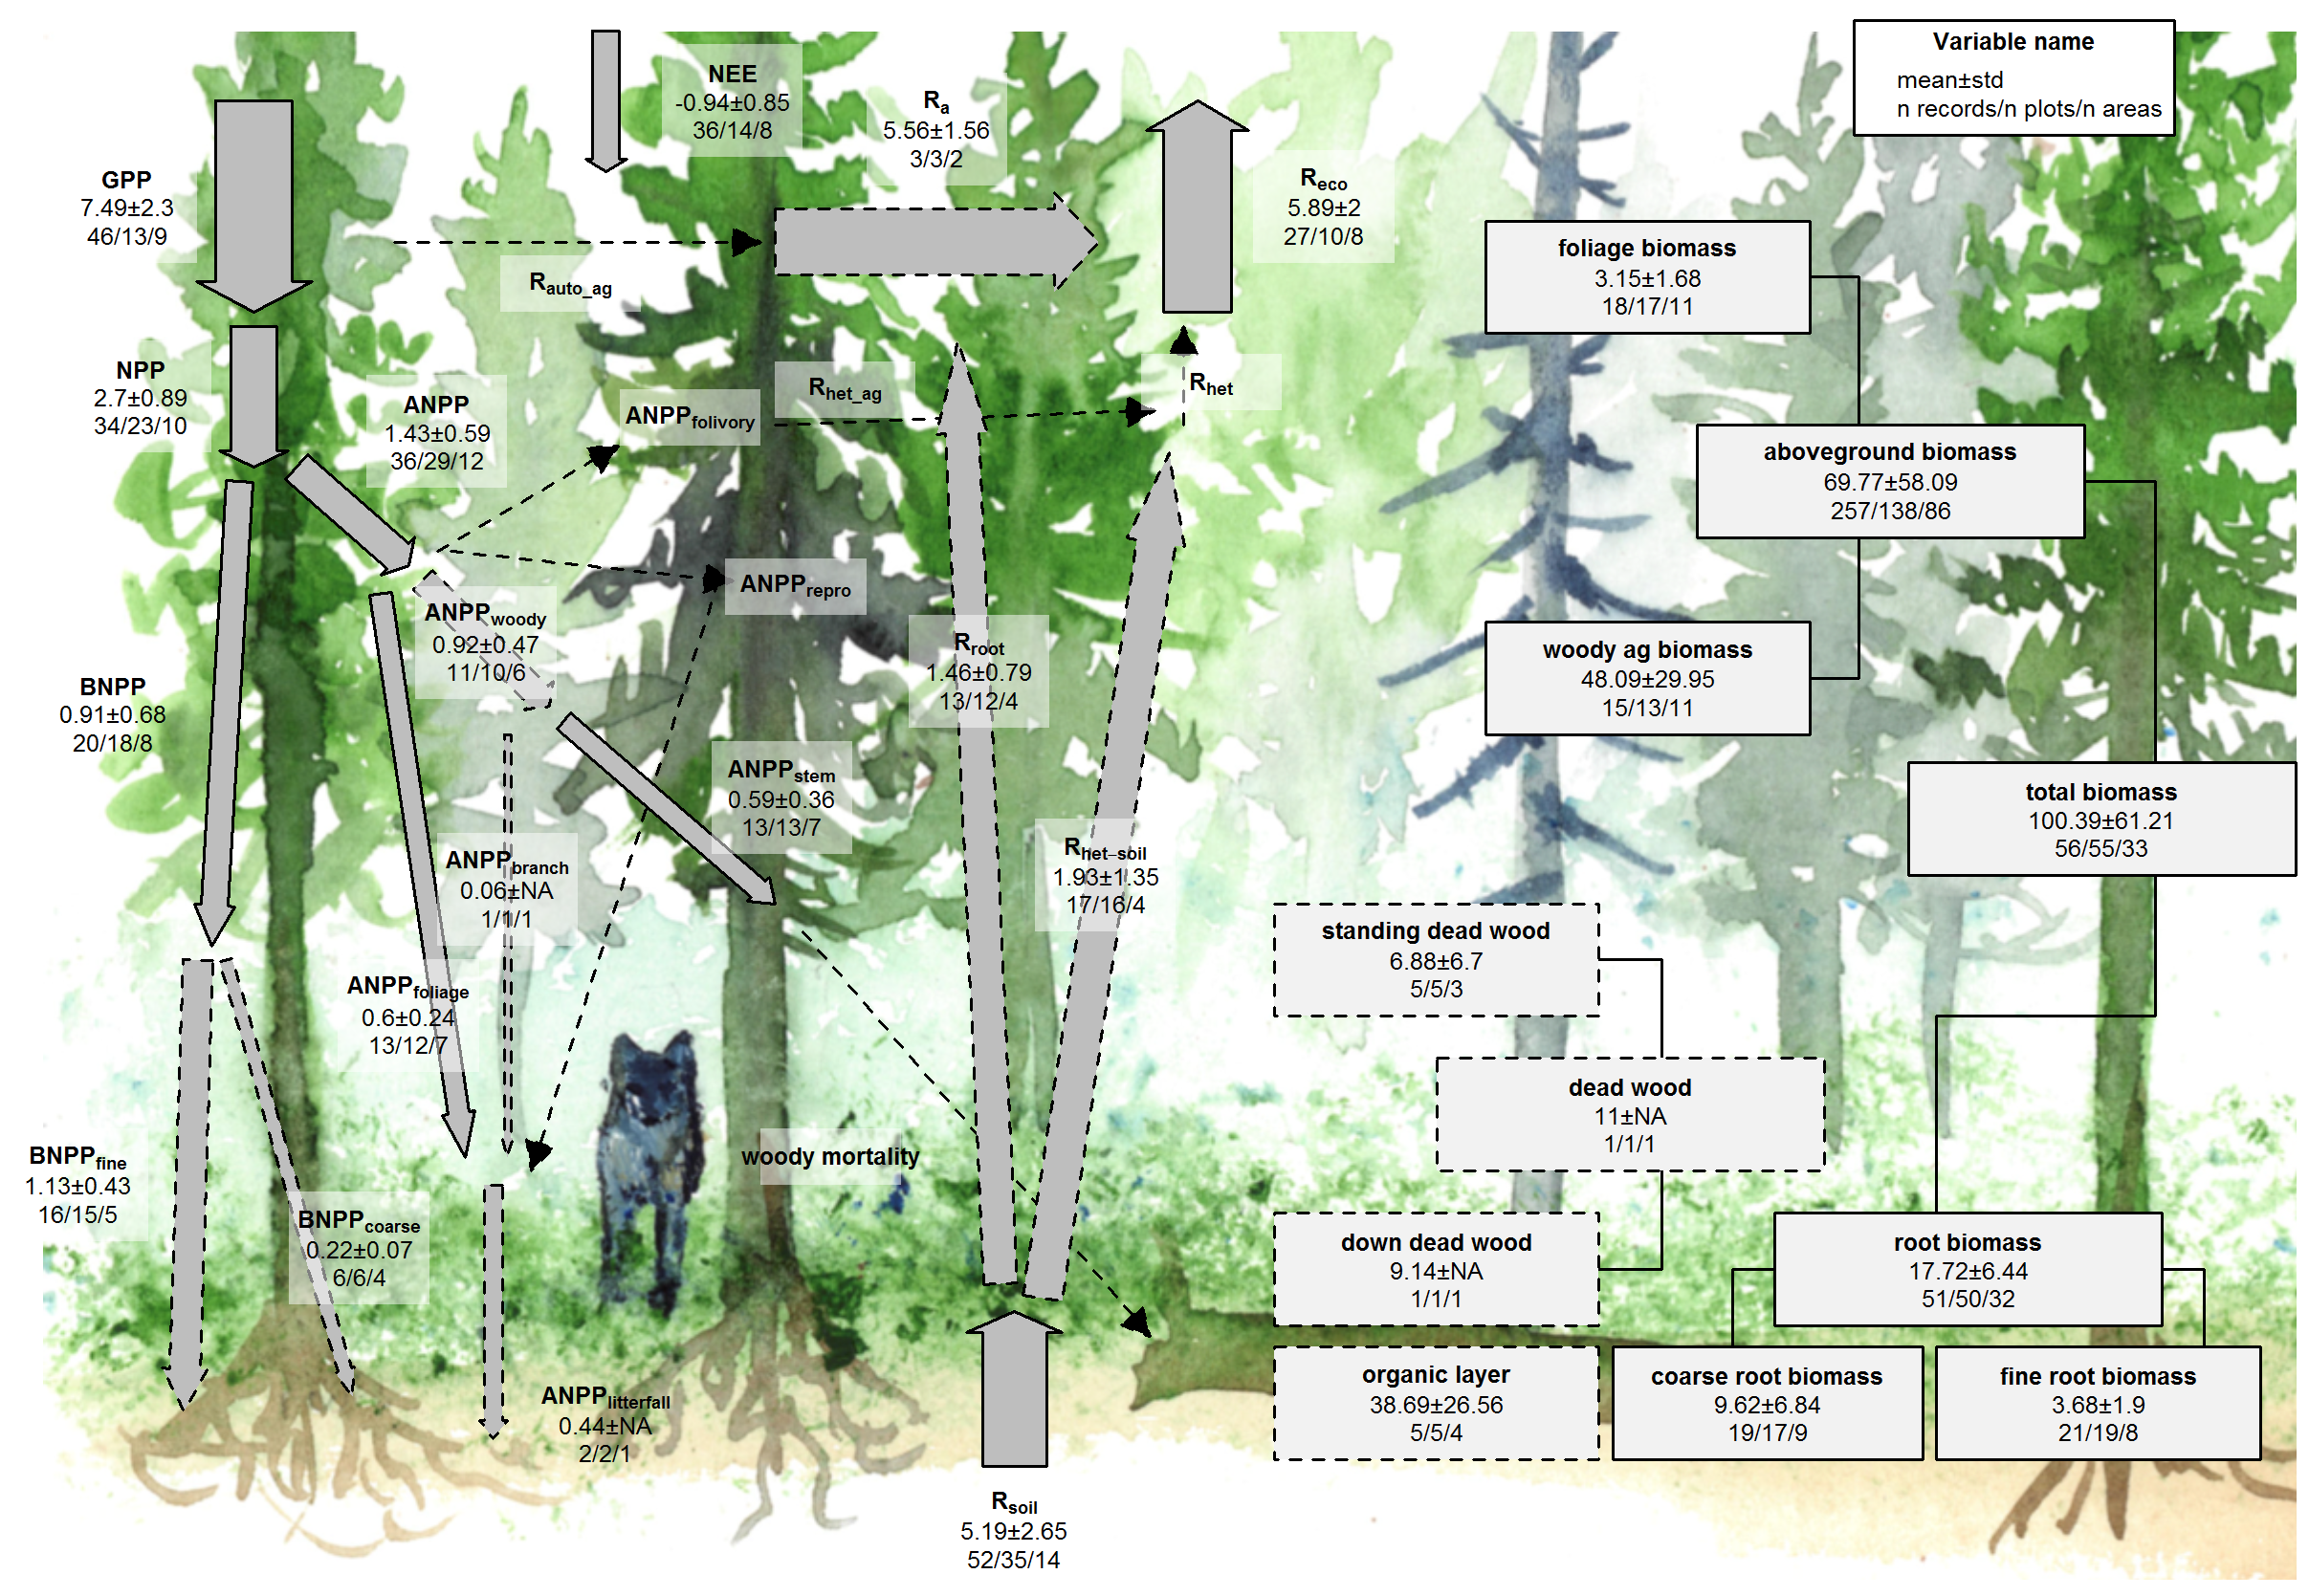
\includegraphics[width=1\linewidth]{/Users/kteixeira/Dropbox (Smithsonian)/GitHub/ForC-db/ForC/figures/C_cycle_diagrams/Diagrams/Boreal conifer MATURE} 

}

\caption{Figure 5 | C cycle diagram for mature boreal conifer forests. All units are Mg C ha$^{-1}$ yr$^{-1}$ (fluxes) or Mg C ha$^{-1}$ (stocks), presented as mean ± std, where geographically distinct areas are treated as the unit of replication.  Arrows indicate fluxes, boxes indicate stocks. Dashed shape outlines indicate variables with records from <7 distinct geographic areas, and dashed arrows indicate fluxes with no data. Arrow size is proportional to the square root of corresponding flux. Asterisk after variable name indicates lack of C cycle closure.}\label{fig:unnamed-chunk-11}
\end{figure}
\end{landscape}

\textbf{check this with final data (based on Table 1):} There were
sufficient data to assess mature forest biome differences for
\textbf{20} flux variables, and significant differences among biomes
were detected for \textbf{14} variables (Table 1). With only
\textbf{one} exception (\(R_{auto}\), which had low sample size;
\textbf{\href{https://github.com/forc-db/ERL-review/issues/40}{issue
40}}), C fluxes were highest in tropical forests, intermediate in
temperate (broadleaf or conifer) forests, and lowest in boreal forests
(Table 1, Figs. 6, S1-S15). Differences between tropical and boreal
forests were always significant, with temperate forests intermediate and
significantly different from one or both. Fluxes tended to be
numerically greater in temperate broadleaf than conifer forests, but the
difference was never statistically significant. This pattern held for
the following variables: ** \(GPP\), \(NPP\), \(ANPP\),
\(ANPP_{woody}\), \(ANPP_{stem}\),\(ANPP_{branch}\), \(ANPP_{foliage}\),
\(ANPP_{litterfall}\), \(M_{woody}\), \(BNPP\), \(R_{eco}\),
\(R_{soil}\), and \(R_{het-soil}\)**. For variables without significant
differences among biomes, the same general trends applied.

The most notable exception to this pattern was \(NEP\), with no
significant differences across biomes but with the largest average in
temperate broadleaf forests, followed by temperate conifer, boreal, and
tropical forests (Figs. 5,S1). Another exception was for
\(BNPP_{root-coarse}\), where all records came from high-biomass forests
in the US Pacific Northwest, resulting in high values for the temperate
conifer biome and no significant differences across biomes (Fig. S10).\\
Thus, C cycling rates generally decreased from tropical to temperate to
boreal forests, with the important exception in the overall C balance
(\(NEP\)).

\begin{figure}[H]

{\centering \includegraphics[width=1\linewidth]{/Users/kteixeira/Dropbox (Smithsonian)/GitHub/ForC-db/ForC/figures/age_trends/for_ERL_review/Flux_age_trends} 

}

\caption{Figure 6 | Age trends and biome differences in some of the major C fluxes: (a) $GPP$, (b) $NPP$, (c) $ANPP$, (d) $R_{soil}$, (e) $R_{eco}$, and (f) $NEP$. Map shows data sources ($x$ and $o$ indicate young and mature stands, respectively). Left plot shows age trends in forests up to 100 years old, as characterized by a linear mixed effects model with fixed effects of age and biome. Solid lines indicate signficant effect of age, non-pareallel lines indicate a significant age x biome interaction. Boxplot illustrates distribution across mature forests, with different letters indicating signifant differences between biomes. Data from biomes that did not meet the sample size criteria (see Methods) are plotted, but lack regression lines (young forests) or test of differences across biomes (mature forests). Individual figures for each flux with sufficient data given in the Supplement (Figs. S1-S15).}\label{fig:unnamed-chunk-12}
\end{figure}

\textbf{check this with final data (based on Table 1):} There were
sufficient data to assess mature forest biome differences for \textbf{9}
stock variables, and significant differences among biomes were detected
for \textbf{6} variables (\textbf{\(B_{tot}\), \(B_{ag}\),
\(B_{ag-wood}\), \(B_{foliage}\), \(B_{root-coarse}\), \(DW_{tot}\)};
Table 1). C stocks had less consistent patterns across biomes (Figs. 7,
S16-S26). In \textbf{four of the six} cases (\textbf{\(B_{tot}\),
\(B_{ag-wood}\), \(B_{root-coarse}\), \(DW_{tot}\)}), temperate conifer
forests were in the highest significance grouping, and boreal forests in
the lowest, with tropical and temperate broadleaf forests in
between--most commonly being significantly different from temperate
conifer but not boreal forests. For \(B_{ag}\), which had by far the
highest sample size, tropical forests exceeded temperate conifer forests
(but not significantly). For \(B_{foliage}\),temperate broadleaf forests
were lowest (again, not significantly). The high values for the
temperate conifer biome were driven by the very high-biomass forests of
the US Pacific Northwest, which are disproportionately represented in
the current version of ForC. Thus, biome differences should be
interpreted more as driven more by geographic distribution of sampling
than by true differences.

\begin{figure}[H]

{\centering \includegraphics[width=1\linewidth]{/Users/kteixeira/Dropbox (Smithsonian)/GitHub/ForC-db/ForC/figures/age_trends/for_ERL_review/Stock_age_trends} 

}

\caption{Figure 7 | Age trends and biome differences in some of the major forest C stocks: (a) aboveground biomass, (b) foliage, (c) fine roots, (d) dead wood. Map shows data sources ($x$ and $o$ indicate young and mature stands, respectively). Left plot shows age trends in forests up to 100 years old, as characterized by a linear mixed effects model with fixed effects of age and biome. Solid lines indicate signficant effect of age, non-pareallel lines indicate a significant age x biome interaction. Boxplot illustrates distribution across mature forests, with different letters indicating signifant differences between biomes. Data from biomes that did not meet the sample size criteria (see Methods) are plotted, but lack regression lines (young forests) or test of differences across biomes (mature forests). Individual figures for each stock with sufficient data given in the Supplement (Figs. S16-S26).}\label{fig:unnamed-chunk-13}
\end{figure}

\hypertarget{c-cycling-in-young-forests}{%
\subsubsection{C cycling in young
forests}\label{c-cycling-in-young-forests}}

Average C cycles for forests \textless100 years old are presented in
Figures 8-11.\\
Both C stocks and fluxes commonly displayed significant trends with
stand age for within-biome analyses (Tables 1, S2, Figs. 6-11, S1-S26;
detailed below).

ForC contained \emph{14} flux variables with sufficient data for
cross-biome analyses of age trends in regrowth forests (see Methods)
(Fig. 6-7 and \textbf{S\#- SI figures including plots for all
variables}). Of these, \emph{9} increased significantly with
log10{[}stand.age{]}: \(GPP\), \(NPP\), \(ANPP\), \(ANPP_{foliage}\),
\(ANPP_{woody}\), \(ANPP_{woody-stem}\), \(BNPP\), \(BNPP_{root-fine}\),
\(R_{eco}\), and net C sequestration (\(NEP\)). The remaining
five--\(ANPP_{woody-branch}\), \(BNPP_{root-coarse}\), \(R_{soil-het}\),
and \(R_{soil-het}\)-\/--displayed no significant relationship to stand
age, although all displayed a positive trend.

Differences in C fluxes across biomes typically paralleled those
observed for mature forests, with C cycling generally most rapid in the
tropics and slowest in boreal forests.\\
The single exception was \(ANPP_{stem}\), for which temperate broadleaf
forests and temperate conifer forests of age
\textgreater{}\emph{\textasciitilde30} had slightly higher flux rates
than tropical forests (\emph{represented by a single chronosequence}).
Notably, the trend of tropical \textgreater{} temperate \textgreater{}
boreal held for \(NEP\) in regrowth forests, in contrast to the lack of
biome differences in \(NEP\) for mature forests (Fig. 6).

There were only \emph{\#\#} flux variables with sufficient data to test
for biome x age interactions: \(ANPP\), \(ANPP_{woody}\),
\(ANPP_{stem}\), \(ANPP_{litterfall}\), and \(BNPP\) (Table S2).
\textbf{(more could be added if age trends become significant after
outliers are resolved)} For three of these (\(ANPP\),
\(ANPP_{litterfall}\), \(BNPP\)), the increase in C flux with age was
steepest increase in tropical forests, followed by temperate and then
boreal forests (Figs S\#). Similarly, \(ANPP_{woody}\) displayed a
steeper increase with age in temperate than boreal boreal forests (no
tropical data for this variable). In contrast, for \(ANPP_{stem}\),
tropical and temperate broadleaf forests had the highest flux rates at
young ages, but were surpassed by temperate conifer forests between ages
20 and 50 (Fig. S6).

(\textbf{this needs to be updated with latest data}) In terms of C
stocks, \emph{10} variables had sufficient data to test for age trends.
\emph{Six} of these---\emph{total biomass, aboveground biomass,
aboveground woody biomass, foliage biomass, root biomass, and coarse
root biomass}--- increased significantly with \(log10[stand.age]\).
\emph{The remaining four displayed non-significant positive trends: fine
root biomass, total dead wood, standing dead wood, and organic layer.}
\emph{(discuss rates of increase)}

\newpage
\begin{landscape}
\begin{figure}[H]

{\centering \includegraphics[width=1\linewidth]{/Users/kteixeira/Dropbox (Smithsonian)/GitHub/ForC-db/ForC/figures/C_cycle_diagrams/Diagrams/Tropical broadleaf YOUNG} 

}

\caption{Figure 8 | C cycle diagram for young tropical broadleaf forests. Presented are observed ranges, where geographically distinct areas are treated as the unit of replication. All units are Mg C ha$^{-1}$ yr$^{-1}$ (fluxes) or Mg C ha$^{-1}$ (stocks). Arrows indicate fluxes, boxes indicate stocks. Dashed shape outlines indicate variables with records from <7 distinct geographic areas, and dashed arrows indicate fluxes with no data. Arrow size is proportional to the square root of corresponding flux.}\label{fig:unnamed-chunk-14}
\end{figure}

\begin{figure}[H]

{\centering \includegraphics[width=1\linewidth]{/Users/kteixeira/Dropbox (Smithsonian)/GitHub/ForC-db/ForC/figures/C_cycle_diagrams/Diagrams/Temperate broadleaf YOUNG} 

}

\caption{Figure 9 | C cycle diagram for young temperate broadleaf forests. Presented are observed ranges, where geographically distinct areas are treated as the unit of replication. All units are Mg C ha$^{-1}$ yr$^{-1}$ (fluxes) or Mg C ha$^{-1}$ (stocks). Arrows indicate fluxes, boxes indicate stocks. Dashed shape outlines indicate variables with records from <7 distinct geographic areas, and dashed arrows indicate fluxes with no data. Arrow size is proportional to the square root of corresponding flux.}\label{fig:unnamed-chunk-15}
\end{figure}

\begin{figure}[H]

{\centering \includegraphics[width=1\linewidth]{/Users/kteixeira/Dropbox (Smithsonian)/GitHub/ForC-db/ForC/figures/C_cycle_diagrams/Diagrams/Temperate conifer YOUNG} 

}

\caption{Figure 10 | C cycle diagram for young temperate conifer forests. Presented are observed ranges, where geographically distinct areas are treated as the unit of replication. All units are Mg C ha$^{-1}$ yr$^{-1}$ (fluxes) or Mg C ha$^{-1}$ (stocks). Arrows indicate fluxes, boxes indicate stocks. Dashed shape outlines indicate variables with records from <7 distinct geographic areas, and dashed arrows indicate fluxes with no data. Arrow size is proportional to the square root of corresponding flux.}\label{fig:unnamed-chunk-16}
\end{figure}

\begin{figure}[H]

{\centering \includegraphics[width=1\linewidth]{/Users/kteixeira/Dropbox (Smithsonian)/GitHub/ForC-db/ForC/figures/C_cycle_diagrams/Diagrams/Boreal conifer YOUNG} 

}

\caption{Figure 11 | C cycle diagram for young boreal conifer forests. Presented are observed ranges, where geographically distinct areas are treated as the unit of replication. All units are Mg C ha$^{-1}$ yr$^{-1}$ (fluxes) or Mg C ha$^{-1}$ (stocks). Arrows indicate fluxes, boxes indicate stocks. Dashed shape outlines indicate variables with records from <7 distinct geographic areas, and dashed arrows indicate fluxes with no data. Arrow size is proportional to the square root of corresponding flux.}\label{fig:unnamed-chunk-17}
\end{figure}
\end{landscape}

\hypertarget{discussion}{%
\subsection{Discussion}\label{discussion}}

ForC v3.0 brought together an unprecedented amount of data to yield an
internally consistent picture of C cycling in the world's major forest
biomes. Carbon cycling rates generally increased from boreal to tropical
regions and with stand age. Specifically, the major C fluxes were
highest in tropical forests, intermediate in temperate (broadleaf or
conifer) forests, and lowest in boreal forests -- a pattern that
generally held for regrowth as well as mature forests (Figs. 6-7). In
contrast to C fluxes, there was little directional variation in mature
forest C stocks across biomes (Figs. 2-5, 7). The majority of flux
variables, together with most live biomass pools, increased
significantly with stand age (Figs. 6-11). Together, these results
indicate that, moving from cold to tropical climates and from young to
old stands, there is a general acceleration of C cycling, whereas C
stocks and \(NEP\) of mature forests are correlated with a different set
of factors.

\hypertarget{c-variable-coverage-and-budget-closure}{%
\subsubsection{C variable coverage and budget
closure}\label{c-variable-coverage-and-budget-closure}}

ForC provides provides unprecedented coverage of most major variables.
\emph{(discuss how this improves upon previous data compilations/ for
which variables does ForC make the greatest difference (e.g., not AGB or
NEP/GPP/Reco, but by far the latest data compilation for dead wood,
{[}variables{]})} \emph{(Noteable holes include: fluxes: R\_auto\_ag,
woody mortality, folivary/ herbivory and respiration of herbivores (and
therefore total R\_het), ANPP\_repro; also fluxes in tropical regrowth
forests)} \emph{For the C stocks considered here, the most poorly
covered is dead wood (none in E hemisphere!), despite a focused effort
on this variable that has resulted in ForC being by far the largest
collection of these data.} Thus, overall, we're lacking coverage of
fluxes to herbivores and higher consumers, along with the woody
mortality and dead wood. Geographically, all variables poorly covered in
Africa and Siberia.

\textbf{notes from Ben on the above par:} Pregitzer and Euskirchen 2004
\url{http://dx.doi.org/10.1111/j.1365-2486.2004.00866.x} ``Aggregated
biome-level estimates of NPP and NEP were higher in intermediate-aged
forests (e.g., 30--120 years), while older forests (e.g., 4120 years)
were generally less productive. The mean NEP in the youngest forests
(0--10 years) was negative (source to the atmosphere) in both boreal and
temperate biomes\ldots Forest age is a highly significant source of
variability in NEP at the biome scale''

Amiro et al.~2010 \url{http://dx.doi.org/10.1029/2010JG001390} Houghton
et al.~2020 \url{https://doi.org/10.1111/gcb.15050}

Turnover: Pugh et al.~2020 \url{http://dx.doi.org/10.5194/bg-2019-491}
Yu et al.~2019 \url{http://dx.doi.org/10.1073/pnas.1821387116}

Human footprint in global forests
\url{http://dx.doi.org/10.1038/nature05847}
\url{http://dx.doi.org/10.1038/nature02619}

Mention consistency (or lack of) with e.g.~GOLUM-CNP?
\url{http://dx.doi.org/10.5194/gmd-11-3903-2018}

In terms of C stocks, there is a paucity of data on dead wood and
organic layer (Pan et al.~?). These can be significant. (\textbf{Note
that we've given a lot of emphasis to dead wood (work by Abby, and also
Jenny), and as a result this work really advances knowledge of dead
wood. We'll want to highlight that here.}) \emph{(give some stats/ cite
figures)}. ForC does not include soil carbon, which is covered by other
efforts (REFS). For fluxes, Fluxnet is the keeper of the best data on
NEE, GPP, Reco (REFS), and SRDB remains the authority on soil
respiration (REFS). ForC includes recent data from both, but is not
continuously integrated. For C is the best source for most of the
subsidiary fluxes: NPP, woody mortality\ldots{}

The C cycle budgets for mature forests (Figs. 2-5) generally
``close''--that is, the sums of component variables do not differ from
the larger fluxes by more than one standard deviation. However, standard
deviations are often large, reflective of significant within-biome
variation. This makes the standard for closure relatively loose.
\emph{Lack of closure, in the few instances where it occurs, is probably
more reflective of differences in the representation of forest types
(e.g., disproportionate representation of US Pacific NW for aboveground
woody biomass relative to AGB; Fig. 4) than of methodological accuracy.}
Thus, overall, a high degree of closure implies that ForC gives a
consistent picture of C cycling within biomes. While these means are
unlikely to be accurate representations of C cycling within any
particular forest, they provide a useful baseline for comparison, always
keeping in mind that sample means do not necessarily represent the true
mean of the entire biome.

\hypertarget{c-cycling-across-biomes}{%
\subsubsection{C cycling across biomes}\label{c-cycling-across-biomes}}

Our analysis reveals a general acceleration of carbon cycling from the
tropics to the high latitudes. For mature forests, this is consistent
with a large body of previous work demonstrating that C fluxes generally
decline with latitude (e.g., Banbury Morgan \emph{et al} n.d.). For
regrowth forests, more rapid accumulation of biomass at lower latitudes
has been well-established (Anderson \emph{et al} 2006, Cook-Patton
\emph{et al} 2020), whereas this is the first study to compare age
trends in deadwood and organic layer across biomes (but see Cook-Patton
\emph{et al} 2020). For most C flux variables, this analysis is the
first to examine flux trends in regrowth forests across biomes (i.e.,
age x biome interaction). Data remain sparse, but for better-represented
variables, we often see faster acceleration of C cycling in the warmer
climates. Further work will be required to explore age x climate
interactions, but our broad-brush overview indicates that C cycling of
regrowth forests is not only higher in the tropics, parallel to fluxes
in mature forests (Banbury Morgan \emph{et al} n.d.), but also that it
accelerates more rapidly with stand age in the tropics, consistent with
more rapid biomass accumulation.

In contrast to C fluxes and accumulation rates in regrowth forests,
stocks\ldots{}

Thus, biome differences should be interpreted more as driven more by
geographic distribution of sampling than by true differences.

Higher NEP in temperate forests -- implications? Invariant NEP in older
forests? This could be built out a bit; thinking of Luyssaert 2008
\url{http://dx.doi.org/10.1038/nature07276} and following papers arguing
about this.

\hypertarget{age-trends-in-c-cycling}{%
\subsubsection{Age trends in C cycling}\label{age-trends-in-c-cycling}}

\emph{(Just some rough notes at this point)}

A relative dearth of data on C cycling in secondary forests,
particularly in the tropics (Anderson-Teixeira et al 2016), is
problematic in that almost 2/3 of the world's forests were secondary as
of 2010 (FAO 2010), implying an under-filled need to characterize
age-related trends in forest C cycling.

Moreover, as disturbances increase ({\textbf{???}}, McDowell \emph{et
al} 2020), understanding the carbon dynamics of regrowth forests will be
increasingly important.

It's also important to understand secondary forest C sequestration to
reduce uncertainty regarding the potential for carbon uptake by regrowth
forests ({\textbf{???}}, Cook-Patton \emph{et al} 2020).

NEP increases with log(age) to 100 --\textgreater{} strongest C sinks
are established secondary forests. (But presumably this exact number is
an artifact; don't over-emphasize.)

\hypertarget{relevance-for-climate-change-prediction-and-mitigation}{%
\subsubsection{Relevance for climate change prediction and
mitigation}\label{relevance-for-climate-change-prediction-and-mitigation}}

The future of forest C cycling ({\textbf{???}}) will shape trends in
atmospheric CO\textsubscript{2} and the course of climate change. For a
human society seeking to understand and mitigate climate change, the
data contained in ForC and summarized here can help to meet two major
challenges.

First, improved representation of forest C cycling in models is
essential to improving predictions of the future course of climate
change. To ensure that models are giving the right answers for the right
reasons, it is important to benchmark against multiple components of the
C cycle that are internally consistent with each other. By making tens
of thousands of records readily available in standardized format, ForC
makes it feasible for the modeling community to draw upon these data to
benchmark models. Integration of ForC with models is a goal (Fer et al.,
in revision).

Second, ForC can serve as a pipeline through which forest science can
inform forest-based climate change mitigation efforts. Such efforts will
be most effective when informed by the best available data, yet it is
not feasible for the individuals and organizations designing such
efforts to sort through literature, often behind paywalls, with data
reported in varying units, terminology, etc. One goal for ForC is to
serve as a pipeline through which information can flow efficiently from
forest researchers to decision-makers working to implement forest
conservation strategies at global, national, or landscape scales. This
is already happening! ForC has already contributed to updating the IPCC
guidelines for carbon accounting in forests {[}IPCC 2019; Requena Suarez
\emph{et al} (2019); Rozendaal et al in prep{]}, mapping C accumulation
potential from natural forest regrowth globally (Cook-Patton \emph{et
al} 2020), and informing ecosystem conservation priorities (Goldstein
\emph{et al} 2020).

\textbf{ForC can complement remote sensing to provide a comprehensive
picture of global forest C cycling.} (\emph{here, discuss what is
well-covered by remote sesnsing, where ForC is useful for calibrating
remote sensing, and what ForC can get that remote sensing can't.}) AGB
is the largest stock, and most of the emphasis is on this variable.
Remote sensing, with calibration based on high-quality ground-based data
(Schepaschenko \emph{et al} 2019, Chave \emph{et al} 2019), is the best
approach for mapping forest carbon (REFS). However, it is limited in
that it is not associated with stand age and disturbance history, except
in recent decades when satellite data can be used to detect forest loss,
gain, and some of their dominant drivers (Hansen \emph{et al} 2013, Song
\emph{et al} 2018, Curtis \emph{et al} 2018). ForC is therefore valuable
in defining age-based trajectories in biomass, as in Cook-Patton
\emph{et al} (2020).

\emph{Remote sensing measurements are increasingly useful for global- or
regional-scale estimates of forest \(GPP\) (Bagdley et al.~2019, (Li and
Xiao 2019)), aboveground biomass (\(B_{ag}\)) (REFS), woody mortality
(}i.e.\emph{, \(B_{ag}\) losses to mortality \(M_{woody}\)) (Clark
\emph{et al} 2004, Leitold \emph{et al} 2018), and to some extent net
ecosystem exchange (\(NEP\)) (REFS).} Other variables, in particular
respiration fluxes, cannot be remotely sensed (({\textbf{???}})), and
efforts such as the Global Carbon Project (\textbf{le quere REF}) and
NASA CMS (\textbf{citation:
\url{https://carbon.nasa.gov/pdfs/CMS_Phase-1_Report_Final_optimized.pdf}
but maybe better to cite open literature, one of the papers listed at
\url{https://cmsflux.jpl.nasa.gov/get-data/publication-data-sets}})
typically compute them as residuals only. (\textbf{Ben, it woudl be
particularly helpful if you could flesh this out some more.})

\textbf{Move to data availability statement, or methods?}: We recommend
that use of ForC data go to the original database, as opposed to using
``off-the-shelf'' values from this publication. This is because (1) ForC
is constantly being updated, (2) analyses should be designed to match
the application, (3) age equations presented here all fit a single
functional form that is not necessarily the best possible for all the
variables.

As climate change accelerates, understanding and managing the carbon
dynamics of forests will be critical to forecasting, mitigation, and
adaptation. The C data in ForC, as summarized here, will be valuable to
these efforts.

\hypertarget{acknowledgements}{%
\subsection{Acknowledgements}\label{acknowledgements}}

All researchers whose data is included in ForC and this analysis. Ian
McGregor for help with the database. Thanks to Norbert Kunert and
{[}Helene's intern{]} for helpful input at an earlier phase. A
Smithsonian Scholarly Studies grant to KAT and HML. WLS grant to KAT.

\hypertarget{data-availability-statement}{%
\subsection{Data availability
statement}\label{data-availability-statement}}

Materials required to fully reproduce these analyses, including data, R
scripts, and image files, are archived in Zenodo (DOI: TBD{]}. Data,
scripts, and results presented here are also available through the
open-access ForC GitHub repository
(\url{https://github.com/forc-db/ForC}), where many will be updated as
the database develops.

\hypertarget{orcid-id}{%
\subsection{ORCID iD}\label{orcid-id}}

Kristina J. Anderson-Teixeira:
\url{https://orcid.org/0000-0001-8461-9713}

\hypertarget{references}{%
\subsection*{References}\label{references}}
\addcontentsline{toc}{subsection}{References}

\hypertarget{refs}{}
\leavevmode\hypertarget{ref-anderson_temperature-dependence_2006}{}%
Anderson K J, Allen A P, Gillooly J F and Brown J H 2006
Temperature-dependence of biomass accumulation rates during secondary
succession \emph{Ecology Letters} \textbf{9} 673--82 Online:
\url{http://www.blackwell-synergy.com/doi/abs/10.1111/j.1461-0248.2006.00914.x}

\leavevmode\hypertarget{ref-anderson-teixeira_forc-dbgroa_2020}{}%
Anderson-Teixeira K, Herrmann V, CookPatton, Ferson A and Lister K 2020
Forc-db/GROA: Release with Cook-Patton et al. 2020, Nature. Online:
\url{https://zenodo.org/record/3983644}

\leavevmode\hypertarget{ref-anderson-teixeira_ctfs-forestgeo_2015}{}%
Anderson-Teixeira K J, Davies S J, Bennett A C, Gonzalez-Akre E B,
Muller-Landau H C, Joseph Wright S, Abu Salim K, Almeyda Zambrano A M,
Alonso A, Baltzer J L, Basset Y, Bourg N A, Broadbent E N, Brockelman W
Y, Bunyavejchewin S, Burslem D F R P, Butt N, Cao M, Cardenas D, Chuyong
G B, Clay K, Cordell S, Dattaraja H S, Deng X, Detto M, Du X, Duque A,
Erikson D L, Ewango C E N, Fischer G A, Fletcher C, Foster R B, Giardina
C P, Gilbert G S, Gunatilleke N, Gunatilleke S, Hao Z, Hargrove W W,
Hart T B, Hau B C H, He F, Hoffman F M, Howe R W, Hubbell S P,
Inman-Narahari F M, Jansen P A, Jiang M, Johnson D J, Kanzaki M, Kassim
A R, Kenfack D, Kibet S, Kinnaird M F, Korte L, Kral K, Kumar J, Larson
A J, Li Y, Li X, Liu S, Lum S K Y, Lutz J A, Ma K, Maddalena D M, Makana
J-R, Malhi Y, Marthews T, Mat Serudin R, McMahon S M, McShea W J,
Memiaghe H R, Mi X, Mizuno T, Morecroft M, Myers J A, Novotny V,
Oliveira A A de, Ong P S, Orwig D A, Ostertag R, Ouden J den, Parker G
G, Phillips R P, Sack L, Sainge M N, Sang W, Sri-ngernyuang K, Sukumar
R, Sun I-F, Sungpalee W, Suresh H S, Tan S, Thomas S C, Thomas D W,
Thompson J, Turner B L, Uriarte M, Valencia R, et al 2015
CTFS-ForestGEO: A worldwide network monitoring forests in an era of
global change \emph{Global Change Biology} \textbf{21} 528--49 Online:
\url{http://onlinelibrary.wiley.com/doi/10.1111/gcb.12712/abstract}

\leavevmode\hypertarget{ref-anderson-teixeira_forc_2018}{}%
Anderson-Teixeira K J, Wang M M H, McGarvey J C, Herrmann V, Tepley A J,
Bond-Lamberty B and LeBauer D S 2018 ForC: A global database of forest
carbon stocks and fluxes \emph{Ecology} \textbf{99} 1507--7 Online:
\url{http://doi.wiley.com/10.1002/ecy.2229}

\leavevmode\hypertarget{ref-anderson-teixeira_carbon_2016}{}%
Anderson-Teixeira K J, Wang M M H, McGarvey J C and LeBauer D S 2016
Carbon dynamics of mature and regrowth tropical forests derived from a
pantropical database (TropForC-db) \emph{Global Change Biology}
\textbf{22} 1690--709 Online:
\url{http://onlinelibrary.wiley.com/doi/10.1111/gcb.13226/abstract}

\leavevmode\hypertarget{ref-baldocchi_fluxnet_2001}{}%
Baldocchi D, Falge E, Gu L, Olson R, Hollinger D, Running S, Anthoni P,
Bernhofer C, Davis K, Evans R, Fuentes J, Goldstein A, Katul G, Law B,
Lee X, Malhi Y, Meyers T, Munger W, Oechel W, Paw K T, Pilegaard K,
Schmid H P, Valentini R, Verma S, Vesala T, Wilson K and Wofsy S 2001
FLUXNET: A New Tool to Study the Temporal and Spatial Variability of
Ecosystem--Scale Carbon Dioxide, Water Vapor, and Energy Flux Densities
\emph{Bulletin of the American Meteorological Society} \textbf{82}
2415--34 Online:
\url{http://journals.ametsoc.org/doi/abs/10.1175/1520-0477(2001)082\%3C2415:FANTTS\%3E2.3.CO;2}

\leavevmode\hypertarget{ref-banbury_morgan_global_nodate}{}%
Banbury Morgan B, Herrmann V, Kunert N, Bond-Lamberty B, Muller-Landau H
C and Anderson-Teixeira K J Global patterns of forest autotrophic carbon
fluxes \emph{Global Change Biology}

\leavevmode\hypertarget{ref-bonan_forests_2008}{}%
Bonan G B 2008 Forests and Climate Change: Forcings, Feedbacks, and the
Climate Benefits of Forests \emph{Science} \textbf{320} 1444--9 Online:
\url{http://www.sciencemag.org/cgi/content/abstract/320/5882/1444}

\leavevmode\hypertarget{ref-bond-lamberty_global_2010}{}%
Bond-Lamberty B and Thomson A 2010 A global database of soil respiration
data \emph{Biogeosciences} \textbf{7} 1915--26 Online:
\url{http://www.biogeosciences.net/7/1915/2010/}

\leavevmode\hypertarget{ref-chave_ground_2019}{}%
Chave J, Davies S J, Phillips O L, Lewis S L, Sist P, Schepaschenko D,
Armston J, Baker T R, Coomes D, Disney M, Duncanson L, Hérault B,
Labrière N, Meyer V, Réjou-Méchain M, Scipal K and Saatchi S 2019 Ground
Data are Essential for Biomass Remote Sensing Missions \emph{Surveys in
Geophysics} \textbf{40} 863--80 Online:
\url{https://doi.org/10.1007/s10712-019-09528-w}

\leavevmode\hypertarget{ref-clark_quantifying_2004}{}%
Clark D B, Castro C S, Alvarado L D A and Read J M 2004 Quantifying
mortality of tropical rain forest trees using high-spatial-resolution
satellite data \emph{Ecology Letters} \textbf{7} 52--9 Online:
\url{https://onlinelibrary.wiley.com/doi/abs/10.1046/j.1461-0248.2003.00547.x}

\leavevmode\hypertarget{ref-cook-patton_mapping_2020}{}%
Cook-Patton S C, Leavitt S M, Gibbs D, Harris N L, Lister K,
Anderson-Teixeira K J, Briggs R D, Chazdon R L, Crowther T W, Ellis P W,
Griscom H P, Herrmann V, Holl K D, Houghton R A, Larrosa C, Lomax G,
Lucas R, Madsen P, Malhi Y, Paquette A, Parker J D, Paul K, Routh D,
Roxburgh S, Saatchi S, Hoogen J van den, Walker W S, Wheeler C E, Wood S
A, Xu L and Griscom B W 2020 Mapping carbon accumulation potential from
global natural forest regrowth \emph{Nature} \textbf{585} 545--50
Online: \url{http://www.nature.com/articles/s41586-020-2686-x}

\leavevmode\hypertarget{ref-curtis_classifying_2018}{}%
Curtis P G, Slay C M, Harris N L, Tyukavina A and Hansen M C 2018
Classifying drivers of global forest loss \emph{Science} \textbf{361}
1108--11 Online:
\url{http://science.sciencemag.org/content/361/6407/1108}

\leavevmode\hypertarget{ref-goldstein_protecting_2020}{}%
Goldstein A, Turner W R, Spawn S A, Anderson-Teixeira K J, Cook-Patton
S, Fargione J, Gibbs H K, Griscom B, Hewson J H, Howard J F, Ledezma J
C, Page S, Koh L P, Rockström J, Sanderman J and Hole D G 2020
Protecting irrecoverable carbon in Earth's ecosystems \emph{Nature
Climate Change} 1--9 Online:
\url{http://www.nature.com/articles/s41558-020-0738-8}

\leavevmode\hypertarget{ref-grassi_key_2017}{}%
Grassi G, House J, Dentener F, Federici S, Elzen M den and Penman J 2017
The key role of forests in meeting climate targets requires science for
credible mitigation \emph{Nature Climate Change} \textbf{7} 220--6
Online: \url{https://www.nature.com/articles/nclimate3227}

\leavevmode\hypertarget{ref-griscom_natural_2017}{}%
Griscom B W, Adams J, Ellis P W, Houghton R A, Lomax G, Miteva D A,
Schlesinger W H, Shoch D, Siikamäki J V, Smith P, Woodbury P, Zganjar C,
Blackman A, Campari J, Conant R T, Delgado C, Elias P, Gopalakrishna T,
Hamsik M R, Herrero M, Kiesecker J, Landis E, Laestadius L, Leavitt S M,
Minnemeyer S, Polasky S, Potapov P, Putz F E, Sanderman J, Silvius M,
Wollenberg E and Fargione J 2017 Natural climate solutions
\emph{Proceedings of the National Academy of Sciences} \textbf{114}
11645--50 Online:
\url{http://www.pnas.org/lookup/doi/10.1073/pnas.1710465114}

\leavevmode\hypertarget{ref-hansen_high-resolution_2013}{}%
Hansen M C, Potapov P V, Moore R, Hancher M, Turubanova S A, Tyukavina
A, Thau D, Stehman S V, Goetz S J, Loveland T R, Kommareddy A, Egorov A,
Chini L, Justice C O and Townshend J R G 2013 High-Resolution Global
Maps of 21st-Century Forest Cover Change \emph{Science} \textbf{342}
850--3 Online:
\url{http://www.sciencemag.org/cgi/doi/10.1126/science.1244693}

\leavevmode\hypertarget{ref-johnson_climate_2018}{}%
Johnson D J, Needham J, Xu C, Massoud E C, Davies S J, Anderson-Teixeira
K J, Bunyavejchewin S, Chambers J Q, Chang-Yang C-H, Chiang J-M, Chuyong
G B, Condit R, Cordell S, Fletcher C, Giardina C P, Giambelluca T W,
Gunatilleke N, Gunatilleke S, Hsieh C-F, Hubbell S, Inman-Narahari F,
Kassim A R, Katabuchi M, Kenfack D, Litton C M, Lum S, Mohamad M,
Nasardin M, Ong P S, Ostertag R, Sack L, Swenson N G, Sun I F, Tan S,
Thomas D W, Thompson J, Umaña M N, Uriarte M, Valencia R, Yap S,
Zimmerman J, McDowell N G and McMahon S M 2018 Climate sensitive
size-dependent survival in tropical trees \emph{Nature Ecology \&
Evolution} \textbf{2} 1436--42 Online:
\url{http://www.nature.com/articles/s41559-018-0626-z}

\leavevmode\hypertarget{ref-krause_large_2018}{}%
Krause A, Pugh T A M, Bayer A D, Li W, Leung F, Bondeau A, Doelman J C,
Humpenöder F, Anthoni P, Bodirsky B L, Ciais P, Müller C,
Murray‐Tortarolo G, Olin S, Popp A, Sitch S, Stehfest E and Arneth A
2018 Large uncertainty in carbon uptake potential of land-based
climate-change mitigation efforts \emph{Global Change Biology}
\textbf{24} 3025--38 Online:
\url{https://onlinelibrary.wiley.com/doi/abs/10.1111/gcb.14144}

\leavevmode\hypertarget{ref-leitold_nino_2018}{}%
Leitold V, Morton D C, Longo M, dos-Santos M N, Keller M and Scaranello
M 2018 El Niño drought increased canopy turnover in Amazon forests
\emph{New Phytologist} \textbf{219} 959--71 Online:
\url{http://doi.wiley.com/10.1111/nph.15110}

\leavevmode\hypertarget{ref-li_mapping_2019}{}%
Li X and Xiao J 2019 Mapping Photosynthesis Solely from Solar-Induced
Chlorophyll Fluorescence: A Global, Fine-Resolution Dataset of Gross
Primary Production Derived from OCO-2 \emph{Remote Sensing} \textbf{11}
2563 Online: \url{https://www.mdpi.com/2072-4292/11/21/2563}

\leavevmode\hypertarget{ref-lutz_global_2018}{}%
Lutz J A, Furniss T J, Johnson D J, Davies S J, Allen D, Alonso A,
Anderson‐Teixeira K J, Andrade A, Baltzer J, Becker K M L, Blomdahl E M,
Bourg N A, Bunyavejchewin S, Burslem D F R P, Cansler C A, Cao K, Cao M,
Cárdenas D, Chang L-W, Chao K-J, Chao W-C, Chiang J-M, Chu C, Chuyong G
B, Clay K, Condit R, Cordell S, Dattaraja H S, Duque A, Ewango C E N,
Fischer G A, Fletcher C, Freund J A, Giardina C, Germain S J, Gilbert G
S, Hao Z, Hart T, Hau B C H, He F, Hector A, Howe R W, Hsieh C-F, Hu
Y-H, Hubbell S P, Inman‐Narahari F M, Itoh A, Janík D, Kassim A R,
Kenfack D, Korte L, Král K, Larson A J, Li Y, Lin Y, Liu S, Lum S, Ma K,
Makana J-R, Malhi Y, McMahon S M, McShea W J, Memiaghe H R, Mi X,
Morecroft M, Musili P M, Myers J A, Novotny V, Oliveira A de, Ong P,
Orwig D A, Ostertag R, Parker G G, Patankar R, Phillips R P, Reynolds G,
Sack L, Song G-Z M, Su S-H, Sukumar R, Sun I-F, Suresh H S, Swanson M E,
Tan S, Thomas D W, Thompson J, Uriarte M, Valencia R, Vicentini A, Vrška
T, Wang X, Weiblen G D, Wolf A, Wu S-H, Xu H, Yamakura T, Yap S and
Zimmerman J K 2018 Global importance of large-diameter trees
\emph{Global Ecology and Biogeography} \textbf{27} 849--64 Online:
\url{https://onlinelibrary.wiley.com/doi/abs/10.1111/geb.12747}

\leavevmode\hypertarget{ref-luyssaert_co2_2007}{}%
Luyssaert S, Inglima I, Jung M, Richardson A D, Reichstein M, Papale D,
Piao S L, Schulze E-D, Wingate L, Matteucci G, Aragao L, Aubinet M, Beer
C, Bernhofer C, Black K G, Bonal D, Bonnefond J-M, Chambers J, Ciais P,
Cook B, Davis K J, Dolman A J, Gielen B, Goulden M, Grace J, Granier A,
Grelle A, Griffis T, Grünwald T, Guidolotti G, Hanson P J, Harding R,
Hollinger D Y, Hutyra L R, Kolari P, Kruijt B, Kutsch W, Lagergren F,
Laurila T, Law B E, Maire G L, Lindroth A, Loustau D, Malhi Y, Mateus J,
Migliavacca M, Misson L, Montagnani L, Moncrieff J, Moors E, Munger J W,
Nikinmaa E, Ollinger S V, Pita G, Rebmann C, Roupsard O, Saigusa N, Sanz
M J, Seufert G, Sierra C, Smith M-L, Tang J, Valentini R, Vesala T and
Janssens I A 2007 CO2 balance of boreal, temperate, and tropical forests
derived from a global database \emph{Global Change Biology} \textbf{13}
2509--37 Online:
\url{http://onlinelibrary.wiley.com/doi/abs/10.1111/j.1365-2486.2007.01439.x}

\leavevmode\hypertarget{ref-mcdowell_pervasive_2020}{}%
McDowell N G, Allen C D, Anderson-Teixeira K, Aukema B H, Bond-Lamberty
B, Chini L, Clark J S, Dietze M, Grossiord C, Hanbury-Brown A, Hurtt G
C, Jackson R B, Johnson D J, Kueppers L, Lichstein J W, Ogle K, Poulter
B, Pugh T A M, Seidl R, Turner M G, Uriarte M, Walker A P and Xu C 2020
Pervasive shifts in forest dynamics in a changing world \emph{Science}
\textbf{368} Online:
\url{https://science.sciencemag.org/content/368/6494/eaaz9463}

\leavevmode\hypertarget{ref-pan_large_2011}{}%
Pan Y, Birdsey R A, Fang J, Houghton R, Kauppi P E, Kurz W A, Phillips O
L, Shvidenko A, Lewis S L, Canadell J G, Ciais P, Jackson R B, Pacala S,
McGuire A D, Piao S, Rautiainen A, Sitch S and Hayes D 2011 A Large and
Persistent Carbon Sink in the World's Forests \emph{Science}
\textbf{333} 988--93 Online:
\url{http://www.sciencemag.org/content/early/2011/07/27/science.1201609.abstract}

\leavevmode\hypertarget{ref-pugh_role_2019}{}%
Pugh T A M, Lindeskog M, Smith B, Poulter B, Arneth A, Haverd V and
Calle L 2019 Role of forest regrowth in global carbon sink dynamics
\emph{Proceedings of the National Academy of Sciences} \textbf{116}
4382--7 Online:
\url{http://www.pnas.org/lookup/doi/10.1073/pnas.1810512116}

\leavevmode\hypertarget{ref-requena_suarez_estimating_2019}{}%
Requena Suarez D, Rozendaal D M A, Sy V D, Phillips O L, Alvarez‐Dávila
E, Anderson‐Teixeira K, Araujo‐Murakami A, Arroyo L, Baker T R, Bongers
F, Brienen R J W, Carter S, Cook‐Patton S C, Feldpausch T R, Griscom B
W, Harris N, Hérault B, Coronado E N H, Leavitt S M, Lewis S L, Marimon
B S, Mendoza A M, N'dja J K, N'Guessan A E, Poorter L, Qie L,
Rutishauser E, Sist P, Sonké B, Sullivan M J P, Vilanova E, Wang M M H,
Martius C and Herold M 2019 Estimating aboveground net biomass change
for tropical and subtropical forests: Refinement of IPCC default rates
using forest plot data \emph{Global Change Biology} \textbf{25} 3609--24
Online: \url{http://onlinelibrary.wiley.com/doi/abs/10.1111/gcb.14767}

\leavevmode\hypertarget{ref-schepaschenko_forest_2019}{}%
Schepaschenko D, Chave J, Phillips O L, Lewis S L, Davies S J,
Réjou-Méchain M, Sist P, Scipal K, Perger C, Herault B, Labrière N,
Hofhansl F, Affum-Baffoe K, Aleinikov A, Alonso A, Amani C,
Araujo-Murakami A, Armston J, Arroyo L, Ascarrunz N, Azevedo C, Baker T,
Bałazy R, Bedeau C, Berry N, Bilous A M, Bilous S Y, Bissiengou P, Blanc
L, Bobkova K S, Braslavskaya T, Brienen R, Burslem D F R P, Condit R,
Cuni-Sanchez A, Danilina D, Torres D del C, Derroire G, Descroix L,
Sotta E D, d'Oliveira M V N, Dresel C, Erwin T, Evdokimenko M D, Falck
J, Feldpausch T R, Foli E G, Foster R, Fritz S, Garcia-Abril A D, Gornov
A, Gornova M, Gothard-Bassébé E, Gourlet-Fleury S, Guedes M, Hamer K C,
Susanty F H, Higuchi N, Coronado E N H, Hubau W, Hubbell S, Ilstedt U,
Ivanov V V, Kanashiro M, Karlsson A, Karminov V N, Killeen T, Koffi J-C
K, Konovalova M, Kraxner F, Krejza J, Krisnawati H, Krivobokov L V,
Kuznetsov M A, Lakyda I, Lakyda P I, Licona J C, Lucas R M, Lukina N,
Lussetti D, Malhi Y, Manzanera J A, Marimon B, Junior B H M, Martinez R
V, Martynenko O V, Matsala M, Matyashuk R K, Mazzei L, Memiaghe H,
Mendoza C, Mendoza A M, Moroziuk O V, Mukhortova L, Musa S, Nazimova D
I, Okuda T, Oliveira L C, et al 2019 The Forest Observation System,
building a global reference dataset for remote sensing of forest biomass
\emph{Scientific Data} \textbf{6} 1--11 Online:
\url{http://www.nature.com/articles/s41597-019-0196-1}

\leavevmode\hypertarget{ref-schimel_observing_2015}{}%
Schimel D, Pavlick R, Fisher J B, Asner G P, Saatchi S, Townsend P,
Miller C, Frankenberg C, Hibbard K and Cox P 2015 Observing terrestrial
ecosystems and the carbon cycle from space \emph{Global Change Biology}
\textbf{21} 1762--76 Online:
\url{http://doi.wiley.com/10.1111/gcb.12822}

\leavevmode\hypertarget{ref-song_global_2018}{}%
Song X-P, Hansen M C, Stehman S V, Potapov P V, Tyukavina A, Vermote E F
and Townshend J R 2018 Global land change from 1982 to 2016
\emph{Nature} \textbf{560} 639--43 Online:
\url{http://www.nature.com/articles/s41586-018-0411-9/}

\leavevmode\hypertarget{ref-taylor_temperature_2017}{}%
Taylor P G, Cleveland C C, Wieder W R, Sullivan B W, Doughty C E,
Dobrowski S Z and Townsend A R 2017 Temperature and rainfall interact to
control carbon cycling in tropical forests ed L Liu \emph{Ecology
Letters} \textbf{20} 779--88 Online:
\url{http://doi.wiley.com/10.1111/ele.12765}

\end{document}
